\documentclass[a4paper,12pt]{article}
 
\usepackage[utf8]{inputenc}
\usepackage[francais]{babel}
\usepackage{graphicx}
\usepackage{amsmath}
\usepackage[font={small,it}]{caption}
\usepackage{setspace}
\usepackage{geometry}

\author{Alexandre Nicaise}
\title{Application mobile : Visualisation 3D de la cornée}
\onehalfspacing
\geometry{hmargin=2.5cm,vmargin=1.5cm}
 
\begin{document}
\maketitle

\newpage
\tableofcontents
\newpage
\section{Introduction}
	\subsection{Département Informatique et Recherche Opérationnelle}
Fondé en 1966, le Département Informatique et Recherche Opérationnelle (DIRO) fut le premier département d’informatique créé au Québec et le troisième au Canada. Le DIRO est situé dans le pavillon André Aisenstadt qui fait partie de l'Université de Montréal (UdeM). L'UdeM a été fondée en 1978 et a été la première Université francophone de Montréal. Elle fait partie des quatre établissements supérieur de Montréal au Québec. Selon la firme QS (Quacquarelli Symonds), l'université de Montréal se classe au 33e rang des meilleures universités du monde en recherche opérationnelle. Elle fait également belle figure en informatique, prenant place parmi le groupe de tête constitué de 150 universités d'excellence. 
		
Durant ce stage, j'ai pu intégrer l'équipe du DIRO dirigé par Jean Meunier. Il s'intéresse à l'analyse et au traitement numérique d’images et de vidéos dans un contexte médical. Ici nous allons plutôt nous intéresser à l'œil et plus précisément à la cornée.

	\subsection{Contexte Biologique}
		\subsubsection{L'œil}
		
L'œil est l'organe de la vision, c'est à dire qu'il capte la lumière afin que le cerveau puisse l'analyser et ainsi interagir avec son environnement. Il possède trois membranes opaques (sclérotique, choroïde et rétinienne) et quatre milieux transparents (cornée, humeur aqueuse, cristallin et humeur vitrée) (Figure : \ref{oeil}). Il est aussi protégé par plusieurs structures annexes comme les paupières, les cils et les sourcils.

\begin{figure}[h]
	\centering
	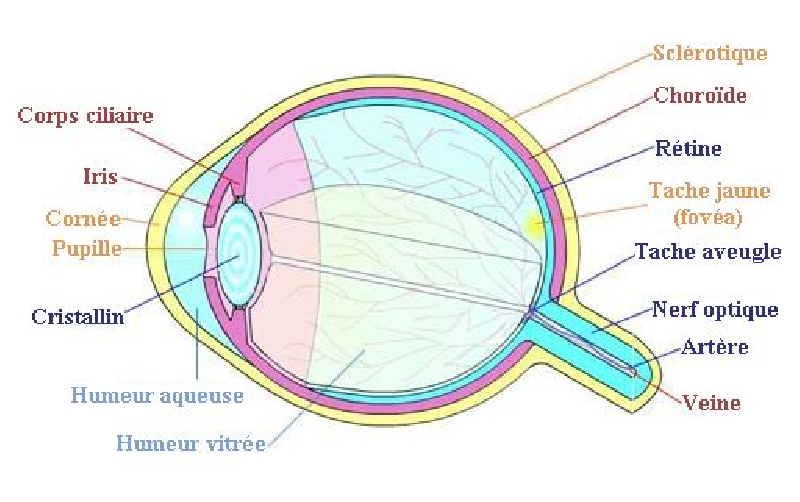
\includegraphics[height=8cm]{oeil.eps} 
	\caption{L'oeil (Gabrielle Bonnet et Gilles Camus)}
	\label{oeil}
\end{figure}

L’œil est souvent comparé à un appareil photo. Il est constitué d'un système optique (un objectif) et d'une surface sensible à la lumière. Le système optique est constitué de la cornée et du cristallin. Il permet de capter les rayons lumineux provenant d'un objet source et de les dévier afin qu'ils convergent en un même point, idéalement situé dans le plan de la surface photosensible. Cette surface est située au sein de la rétine et est recouverte de cellules appelées photorécepteurs. Les photorécepteurs sont soit des cônes permettant la vision diurne, soit des bâtonnets permettant la vision nocturne. Ensuite nous quittons le domaine de l'appareil photo et passons dans le traitement de l'information. Les photorécepteurs créent un influx nerveux en réaction à leur exposition aux rayons lumineux. L'influx nerveux passe dans le nerf optique pour atteindre l'aire visuelle du cerveau. Le cerveau se charge ensuite de déchiffrer l'information contenue dans l'influx nerveux afin de permettre l'interaction avec l'environnement. (Figure : \ref{fig:Vision})

\begin{figure}[h]
	\centering
	\includegraphics[height=10cm]{Vision.eps} 
	\caption{Présentation du mécanisme de la vision}
	\label{fig:Vision}
\end{figure}


Ici nous nous intéresserons plus à un des éléments du système optique : la cornée.



		\subsubsection{La cornée}

La cornée est un composant oculaire essentiel au fonctionnement de la vision: elle est la première structure que rencontre la lumière qui pénètre l’œil. Son rôle principal est de faire converger les rayons lumineux incidents vers le cristallin, avant de rencontrer la rétine et d'enclencher la cascade visuelle en créant l'influx nerveux. Cette convergence est représenter par le pouvoir optique de la cornée. Le pouvoir optique, aussi appelé pouvoir réfractif ou de vergence, représente le degrés de réfraction des rayons lumineux lors de la traversé d'un milieux. Il est représenté par une unité de mesure appelé dioptrie et qui est une unité de vergence homogène à l'inverse de la longueur.  Une valeur négative montre une divergence alors qu'une valeur positive montre une convergence. La cornée assure les deux tiers du pouvoir optique des structures oculaires, le tiers restant étant dévolu au cristallin. Ce pouvoir optique découle de deux caractéristiques de la cornée : \vspace{0.15cm}
\begin{itemize}\setlength{\itemsep}{1mm}
	\item[$\bullet$] une courbure plus importante que celle du cristallin non accommodé. Les accommodations du cristallin sont des modification effectué sur celle-ci afin de modifier la réfraction du cristallin et ainsi amélioré la netteté de l'image.
	\item[$\bullet$] le contact avec l'air ambiant, offrant la plus grande différence d'indice de réfraction aux rayons lumineux incidents par rapport au cristallin qui est au contact d'un liquide et donc avec un indice de réfraction moindre. 
\end{itemize}

 \vspace{0.5cm}
La cornée est un tissu non vascularisé et transparent. C'est une coupole hémisphérique au contact direct de l'air. Elle couvre environ un cinquième de la surface de l’œil et a un diamètre d'environ 12 mm. La cornée est légèrement plus épaisse en périphérie (0.6 mm) par rapport à son centre (0.5 mm). Pour qualifier l'épaisseur, j'utiliserai le terme de pachymétrie. Le rayon de courbure est d'environ 6.5 mm pour la surface postérieure et varie de 7 à 9 mm pour la surface antérieure. La transparence de la cornée et la régularité de la courbure permet une transmission sans perte préjudiciable en quantité et qualité de l'information lumineuse. Seulement 4\% à 6\% de la lumière incidente est réfléchie par la surface cornéenne. Cette propriété de réflexion est mise à profit pour la réalisation de l'examen de topographie cornéenne.

\begin{figure}[h]
	\centering
	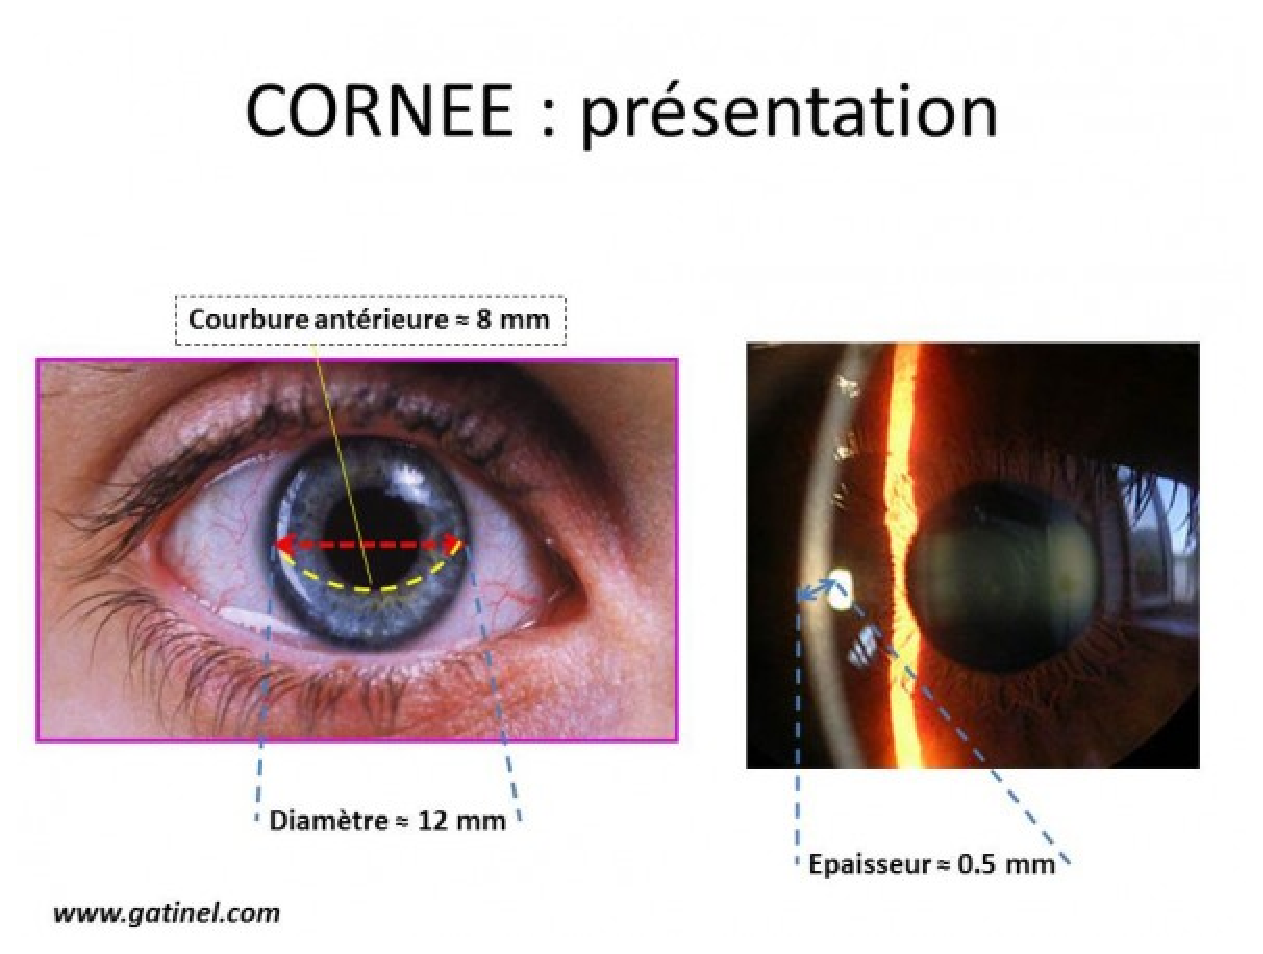
\includegraphics[width=15cm, trim=0cm 0cm 0cm 3cm, clip]{CorneePresentation.eps} 
	\caption{Présentation de la cornée. L'image de gauche montre le diamètre et la courbure moyenne de la cornée. L'image de droite montre l'épaisseur entre la surface antérieure et la surface postérieure aussi appelé pachymétrie.}
\end{figure}


		\subsubsection{Topographie de la cornée}
La topographie permet de recueillir des informations relatives à la courbure ou au relief (élévation) de la cornée, grâce à la projection et l'analyse du reflet d'un motif lumineux éclairant ou balayant la cornée. Les images recueillies sont analysées de façon automatisée et des cartes en couleurs sont fournies au praticien pour interprétation. La topographie est courante lors d'un examen ophtalmologique, pour réaliser un diagnostic ou un suivi. En effet, des déformations peuvent être liées par exemple, à des pathologies, des traumatismes, une chirurgie, ou simplement à l'âge. Dès lors, la possibilité d'estimer et de caractériser cette déformation permet d'apporter une information pertinente au médecin pour aider à son diagnostic. 

Lors de mon stage, j'ai utilisé des données obtenues via l'appareil Orbscan II (Figure 2) qui permet de mesurer l'élévation de la cornée. Il est capable de mesurer la partie antérieure ainsi que la partie postérieure de la cornée avec une marge d'erreur de l'ordre du micron. Les données peuvent se présenter sous la forme d'une grille 101x101 contenant les valeurs d'élévation qui ont été prises toute les 0.1 mm. A partir de cette matrice d'élévation, il est possible de construire des maillages qui seront utilisés par la suite pour la visualisation en 3 dimensions de la cornée. 

La cornée étant presque sphérique, un moyen simple et efficace de visualiser l'aspect de sa surface est d'utiliser une référence sphérique afin d'observer les différences entre la référence et la cornée. 
\vspace{0.25cm}

\begin{figure}[h]
	\centering
	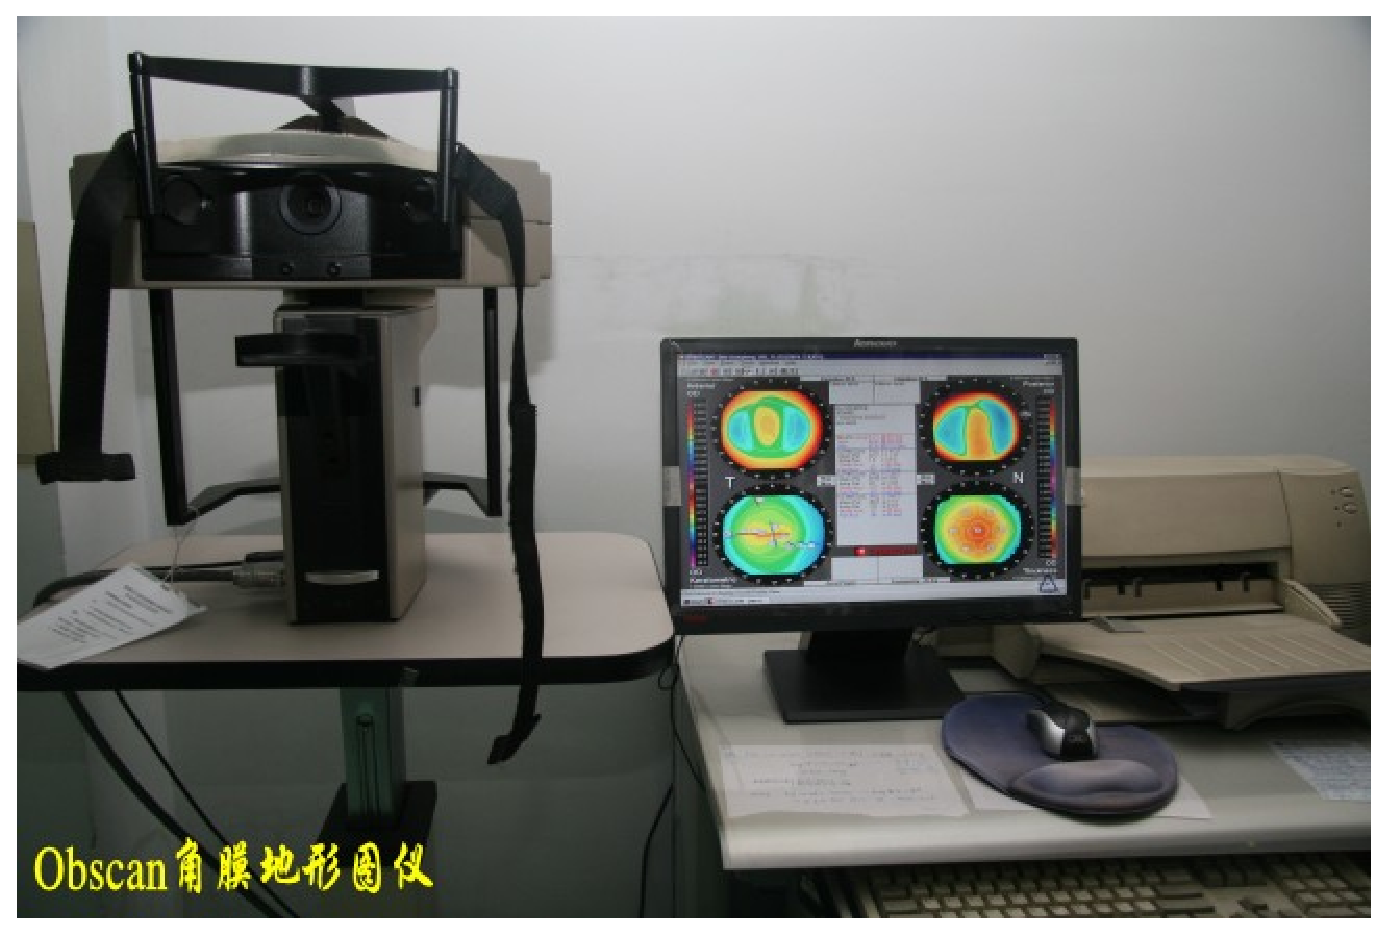
\includegraphics[ width=12cm]{Obscan.eps}
	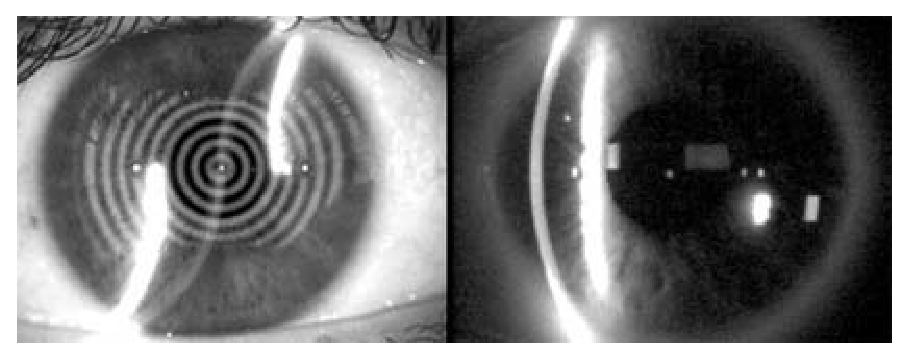
\includegraphics[width=12cm]{orbscanPrincipes.eps} 
	\caption{Orbscan II. L'image du dessus présente l'appareil. Les autres images présentent le principe de l'orbscan. Il associe la réflexion du disque de Placido (à droite) sur la cornée au balayage de l'œil par une fente lumineuse (à gauche).}
\end{figure}

\subsubsection{"Best Fit Sphere" (BFS)}

Afin d'affiner leurs diagnostics les praticiens ont besoin de mieux connaître l'aspect de la surface de la cornée. La cornée étant presque sphérique, il est possible de la comparer en faisant la différence des deux. Pour cela, on calcule la "Best Fit Sphere" (BFS) qui est la sphère qui correspond le mieux à la matrice d'élévation, puis on effectue la différence entre les deux surfaces. Cette différence va permettre de construire une carte semblable à celles utilisées par les géologues pour représenter les reliefs de la terre. En effet, afin de mettre en évidence ces "reliefs" ces différences sont représentées selon un jeu de couleur standard. Les différences positives seront associer des couleurs chaudes (points à l'extérieur de la BFS) et les différences négatives (points à l'intérieur de la BFS) à des couleurs froides. Il est nécessaire de calculer deux BFS différentes, une pour la face antérieure et une pour la face postérieure. 
\vspace{0.5cm}

La BFS est calculée en minimisant la somme des distances au carré entre la sphère et chaque point de la cornée, ce qui donne l'expression suivante à minimiser :
\vspace{0.25cm}

$ f(c,R) = \overset{n}{\underset{k=1}{\sum}} \sqrt{(x_k-x_c)^2 + (y_k-y_c)^2 + (z_k-z_c)^ 2} - R^2$
\vspace{0.25cm}

Avec k un point de la cornée, c le centre de la BFS, R son rayon et n le nombre de point de la cornée.

\vspace{0.5cm}
L'association d'image représentée par la figure~\ref{fig:CorneaConstruct} permet la visualisation des différentes étapes de construction de la carte topographique de la cornée. 

\begin{figure}[h]
	\centering
	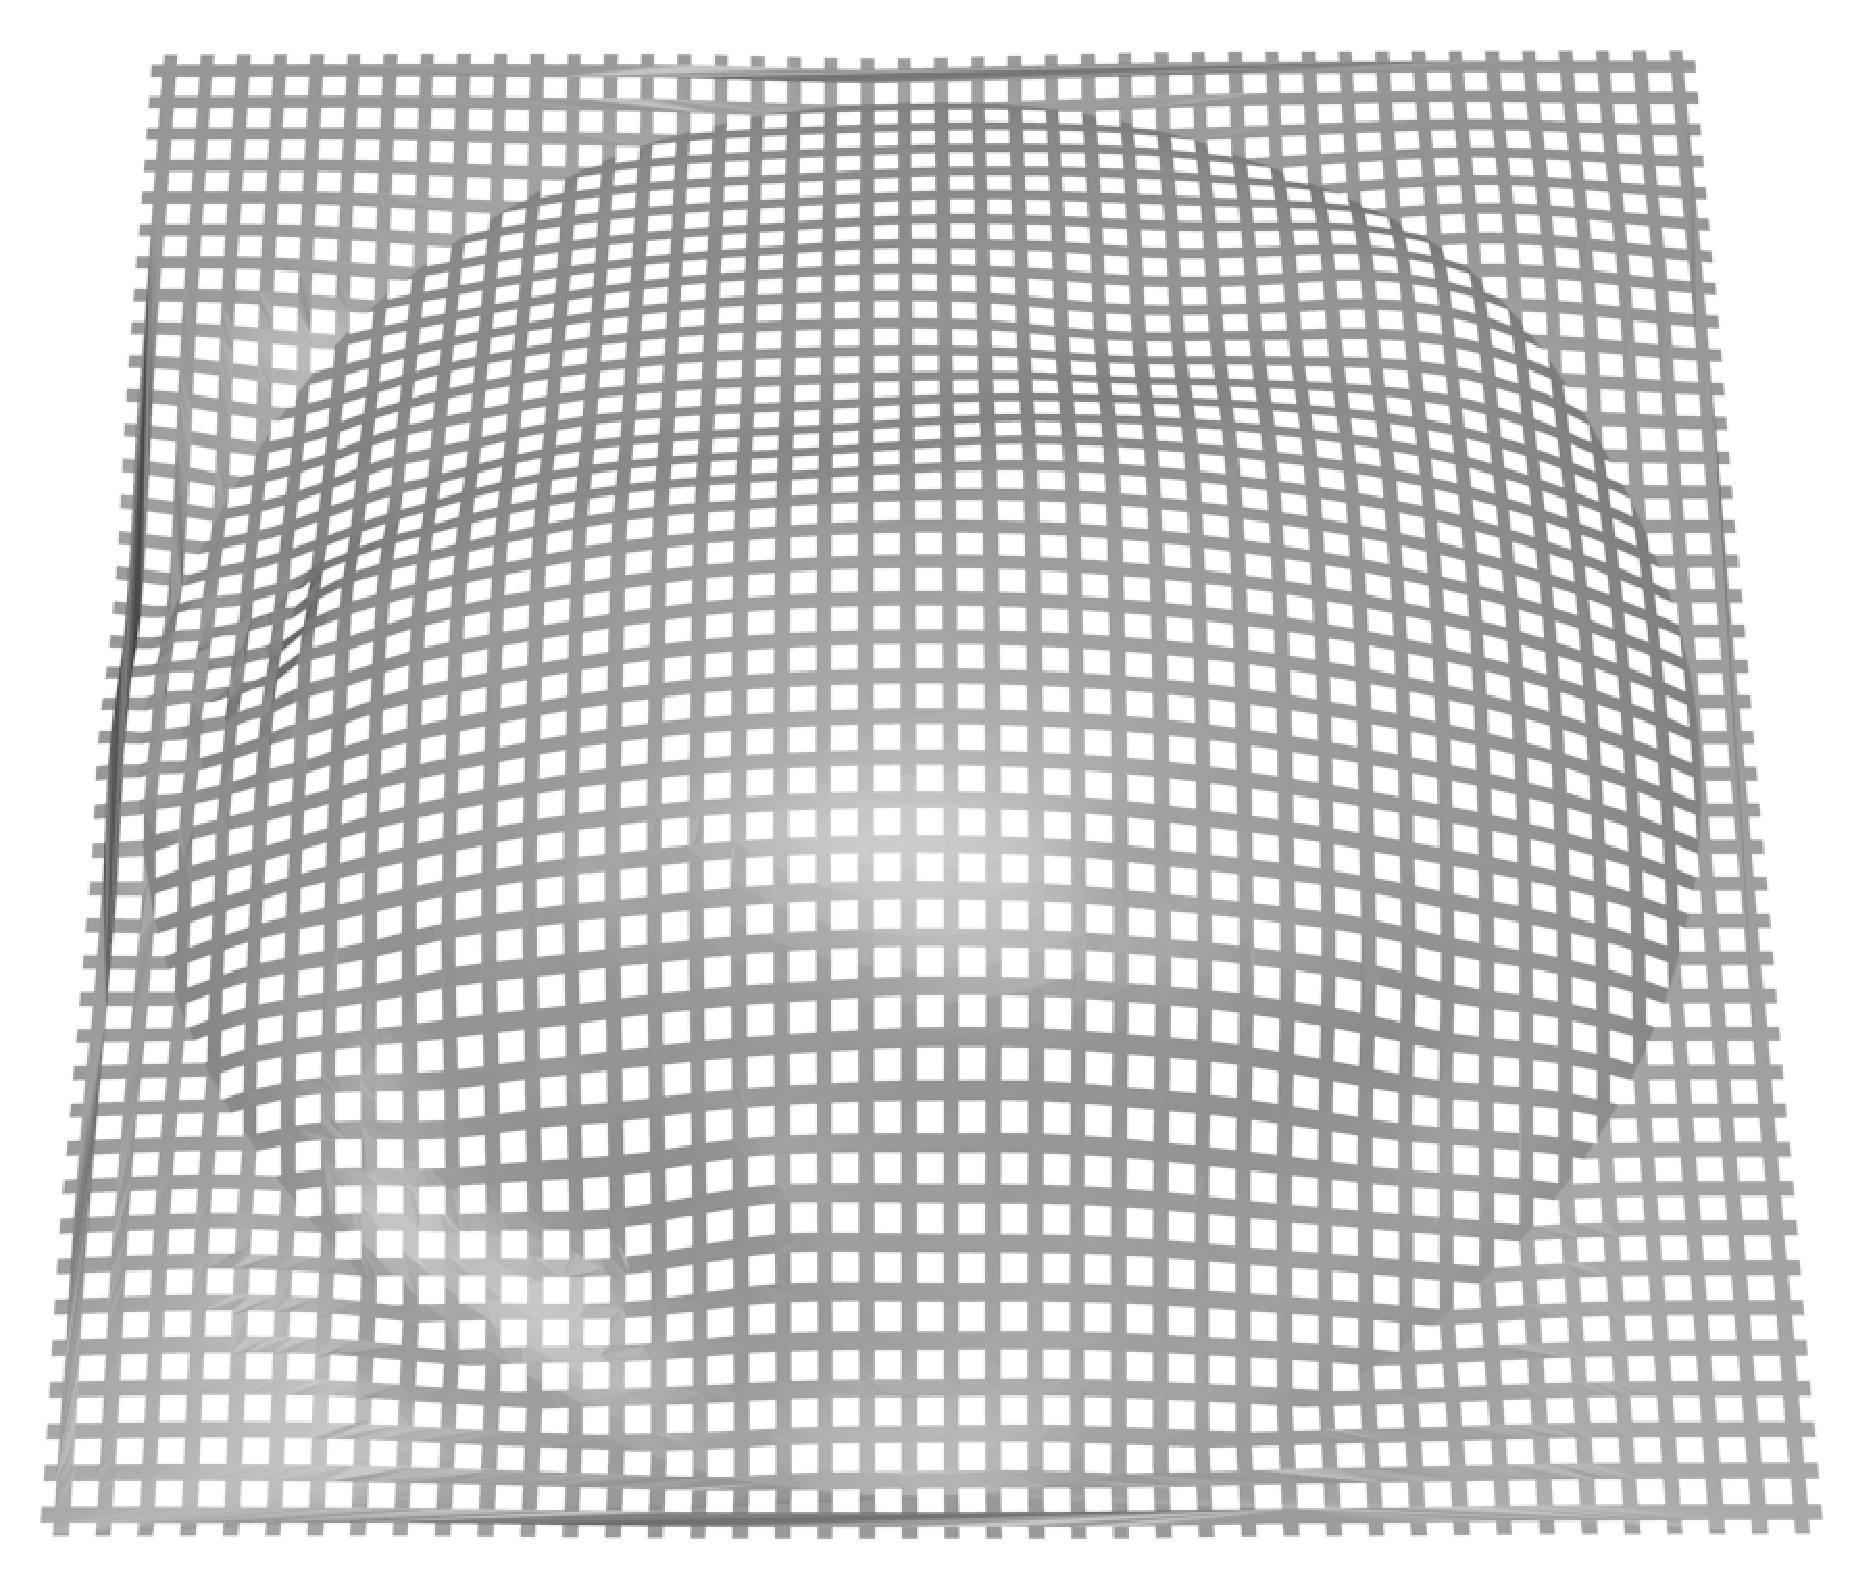
\includegraphics[ width=4.5cm]{bfs.eps}
	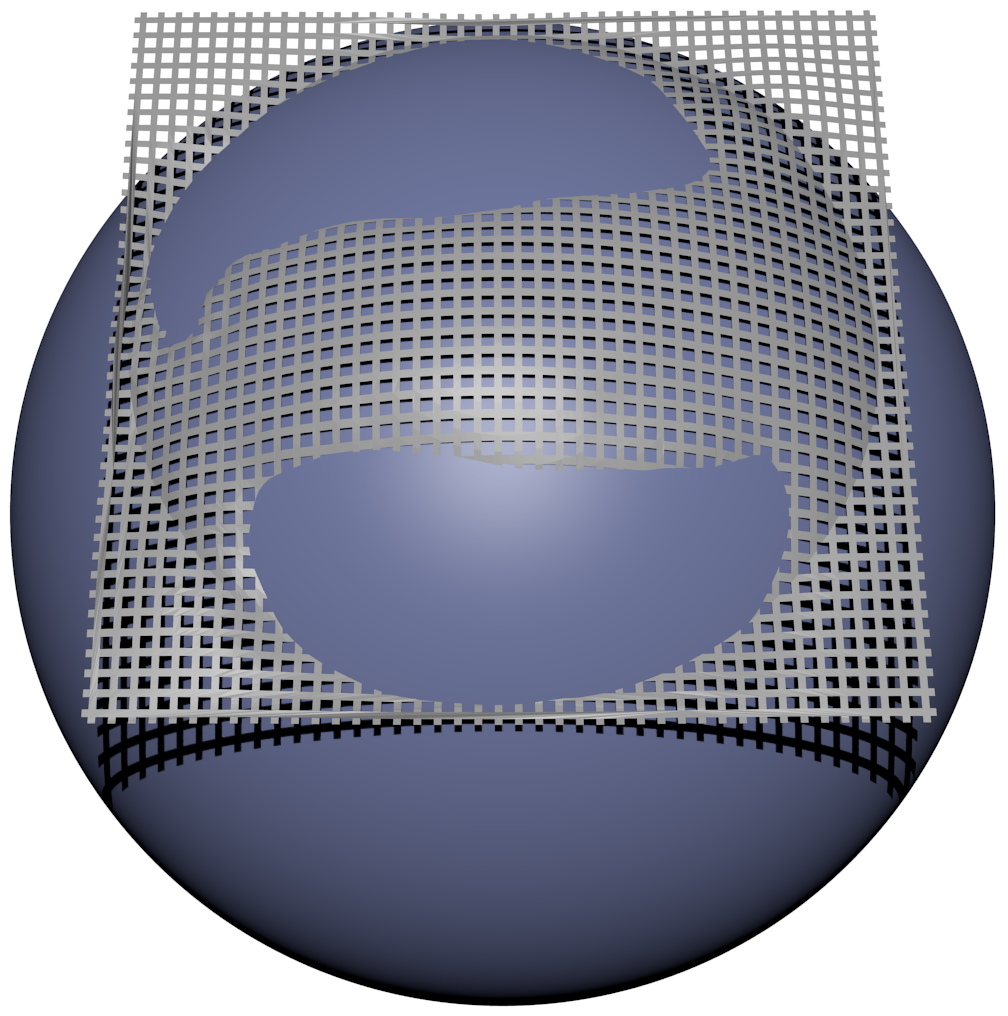
\includegraphics[ width=4.5cm]{carteElevation.eps}
	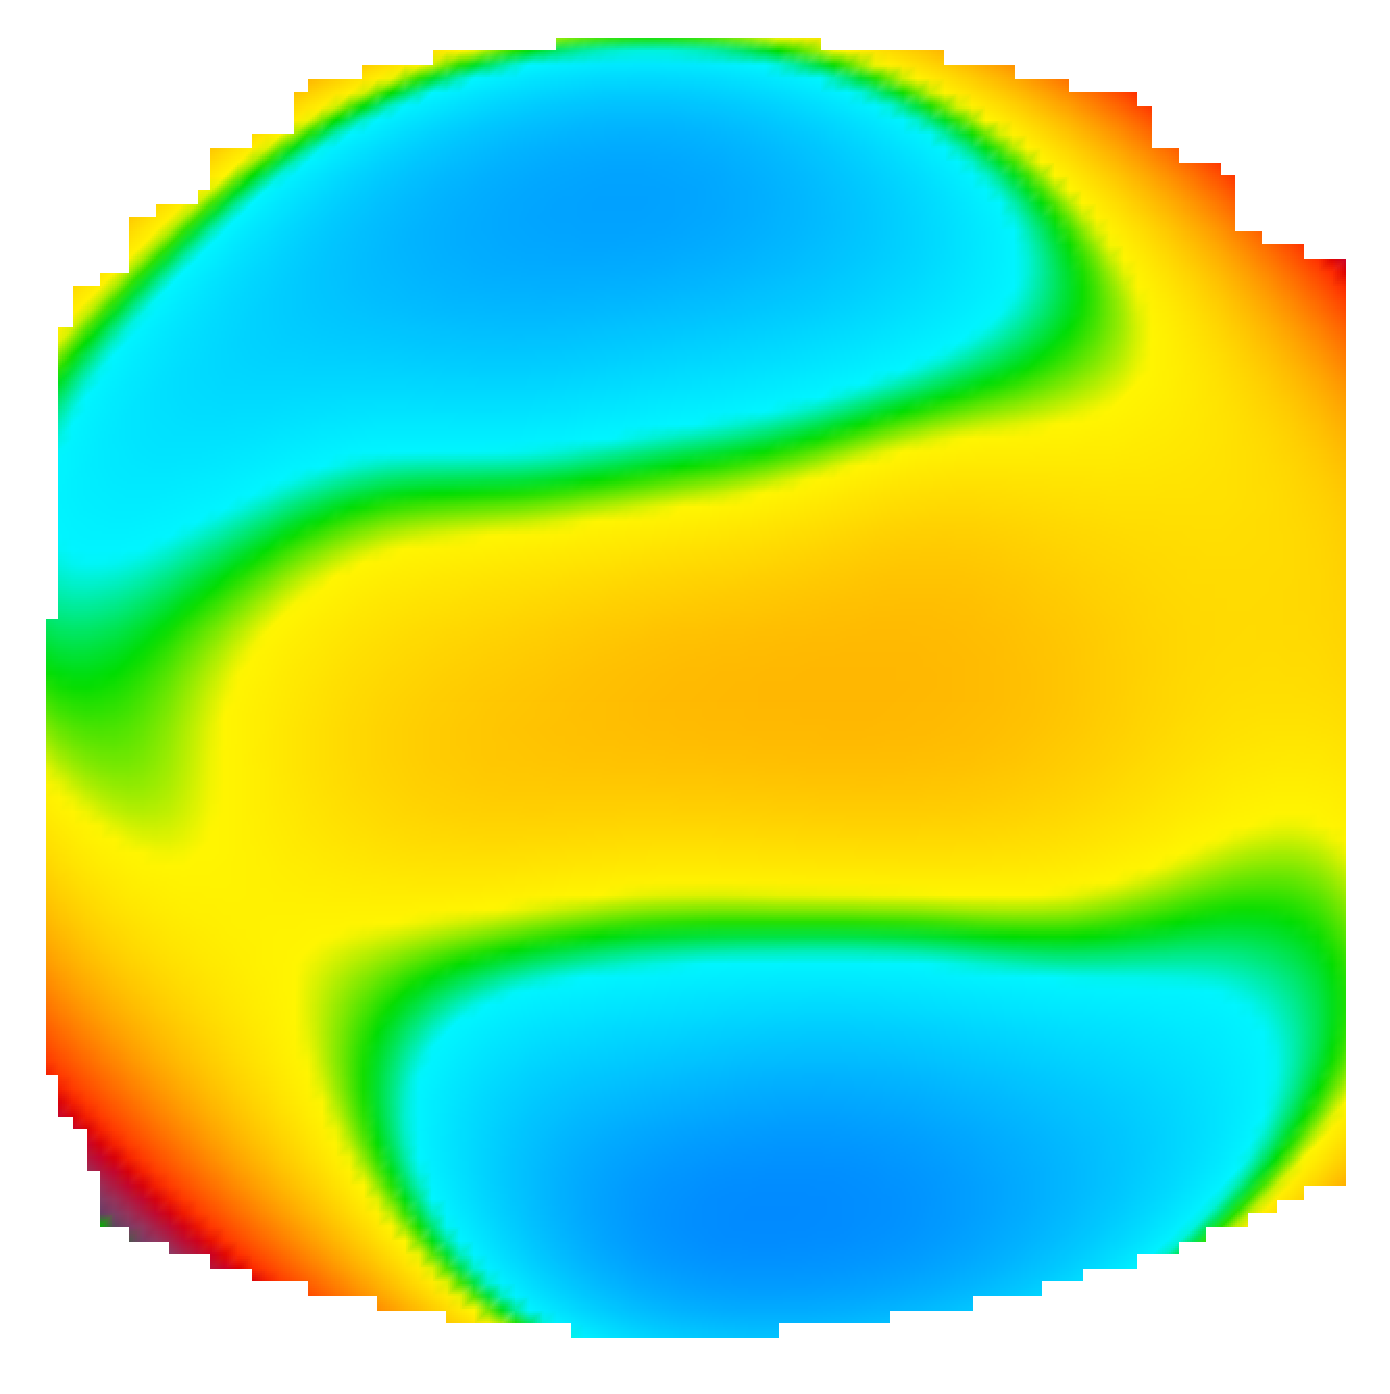
\includegraphics[ width=4.5cm]{carteElevationcouleur.eps}
	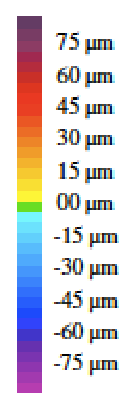
\includegraphics[ height=4cm]{pallette.eps}
	\caption{Présentation de la construction de la carte de couleur d'une cornée. A gauche nous pouvons voir la matrice 101x101 obtenue par l'orbscan. L'image suivante est la superposition de la BFS (Best Fit Sphere) et de cette matrice. La troisième image est l'ajout des couleurs afin de visualiser les relief de la cornée selon une palette de couleur située juste à côté. On peut voir que les couleurs froides sont situées en-dessous de la BFS, les couleurs chaudes au-dessus et le vert symbolise le passage à 0.}
	\label{fig:CorneaConstruct}
\end{figure} 

\newpage
	\subsection{Problématique du stage}
Le but de mon stage a été de construire une application mobile permettant de visualiser une cornée en trois dimensions. Ce projet intéresse beaucoup les praticiens de l'hôpital, car cela faciliterait l'accès aux cartes topographiques des cornées de leurs patients. En effet, le praticien pourra changer de cornée voir de dossier de patient plus facilement que si les cartes était en papier et une tablette est plus pratique à transporter qu'un ordinateur. Ce projet a été débuté l'année dernière par Ouri Saban un étudiant du master CCI. Mon but a été d'utiliser une bibliothèque appelée Visual Tool Kit (VTK), afin de visualiser la cornée sur des plateformes mobile.

%%%%%%%%%%%%%%%%%%%%%%%%%%%%%%%%%%%%%%%%%%%% Math Meth %%%%%%%%%%%%%%%%%%%%%%%%%%%%%%%%%%%%%%%%%%%%%

\newpage
\section{Matériels et méthodes}
	\subsection{Données disponibles}
Pour mes tests, je me suis servi d'un document texte fournis par Arnaud Polette qui contient toutes les informations de la cornée obtenue par le biais de l'Orbscan. Elles sont sous la forme de plusieurs matrices 101x101 contenant les valeurs d'élévations et dont les valeurs de X et de Y sont situées de -5 à +5 mm séparées par des pas de 0.1 mm.

\vspace{0.25cm}
\parindent=0em Ces matrices permettent de visualiser : %empêche l'espace avant le nouveau paragraphe
\begin{itemize}\setlength{\itemsep}{1mm}
	\item[$\bullet$] la face postérieure 
	\item[$\bullet$] la face antérieure
	\item[$\bullet$] la différence entre la postérieure et la BFS
	\item[$\bullet$] la différence entre la antérieure et la BFS
	\item[$\bullet$] la pachymetrie
	\item[$\bullet$] la tangentielle de la face antérieure
	\item[$\bullet$] la tangentielle de la face postérieure
\end{itemize}

\vspace{0.25cm}
\parindent=1.5em
 Pour réaliser la visualisation en 3D de la cornée, je me suis servi des matrices représentant la face antérieure, la face postérieure, la BFS et la pachymetry. Les rayons et centres des sphères utilisées sont déduites de ces matrices. Nous avons donc tout les éléments nécessaire à la visualisation en trois dimension de la cornée.

	\subsection{VTK (Visualisation Toll Kit)}
	VTK est une librairie construite par Kitware qui est constitué de classe en C++ avec plusieurs couches de surfaces interprétées incluant le Tcl/Tk, Java et Python. Elle est très utilisé par les chercheurs et permet l'infographie en trois dimension, le traitement d'image et la visualisation. Nous avons choisi VTk car nous avons été séduits par une application open-source utilisant VTK appelé KIWIVIEWER qui fonctionne aussi bien sur android, que sur ios. De plus, VTK possède de nombreux exemples qui permettent d'apprendre à l'utiliser.
	
\vspace{0.25cm}
\parindent=0em Pour la visualisation j'ai utilisé les éléments de vtk suivants :
\begin{itemize}\setlength{\itemsep}{1mm}
	\item[$\bullet$] vtkPoints	$\rightarrow$ stocke les coordonnées obtenue par le biais des matrices d'élévation 
	\item[$\bullet$] vtkFloatArray $\rightarrow$ affecte un "scalar" à une coordonnée. Un scalar est une valeur qui permettra la représentation sous forme de couleurs. Ici nous utiliserons les valeurs d'élévations.
	\item[$\bullet$] vtkCellArray $\rightarrow$ construit le maillage. Le maillage est la représentation d'une surface (ici la cornée) en la subdivisant en un ensemble de polygones. Il est composé de sommets,  connectés les uns aux autres par des faces ou facettes de forme polygonale. Lorsque toutes les faces sont des triangles, on parle de maillage triangulaire (trimesh), ou de triangulation selon les domaines. Les maillages par quadrilatères sont aussi très courants. En 3 !! trois/3D !! dimensions, il est aussi possible d'utiliser des maillages volumiques, qui relient les sommets par des tétraèdres, des hexaèdres et des prismes. Ici, j'ai utilisé le maillage triangulaire. 
	\item[$\bullet$] vtkPolyData $\rightarrow$ regroupe les objets vtkPoints, vtkFloatArray et vtkCellArray.
	\item[$\bullet$] vtkPolyMapper	$\rightarrow$ permet la transformation de la structure de données contenue dans vtkPolyData en primitives OpenGL. Les primitives OpenGL sont des points, des lignes ou des triangles. Il permet aussi l'association de couleurs qui peut être contrôler en spécifiant une table de couleurs (lookup table) et un intervalle.
	\item[$\bullet$] vtkActor $\rightarrow$ sert à positionner et orienter l'objet, à le colorer et choisir des propriétés graphiques. 
	\item[$\bullet$] vtkRenderer $\rightarrow$ lance les algorythmes nécessaires au rendu de l'objet
	\item[$\bullet$] vtkRenderWindow $\rightarrow$ spécifie une fenêtre qui affiche le rendu
	\item[$\bullet$] vtkRenderWindowInteractor $\rightarrow$ permet l'intéraction avec l'objet en faisant bouger la caméra.
\end{itemize}
 \vspace{0.25cm}
La figure~\ref{fig:VTKMeth} permet de visualiser la construction de la carte d'élévation (mapper) à partir d'une matrice.

\begin{figure}[h]
	\centering
	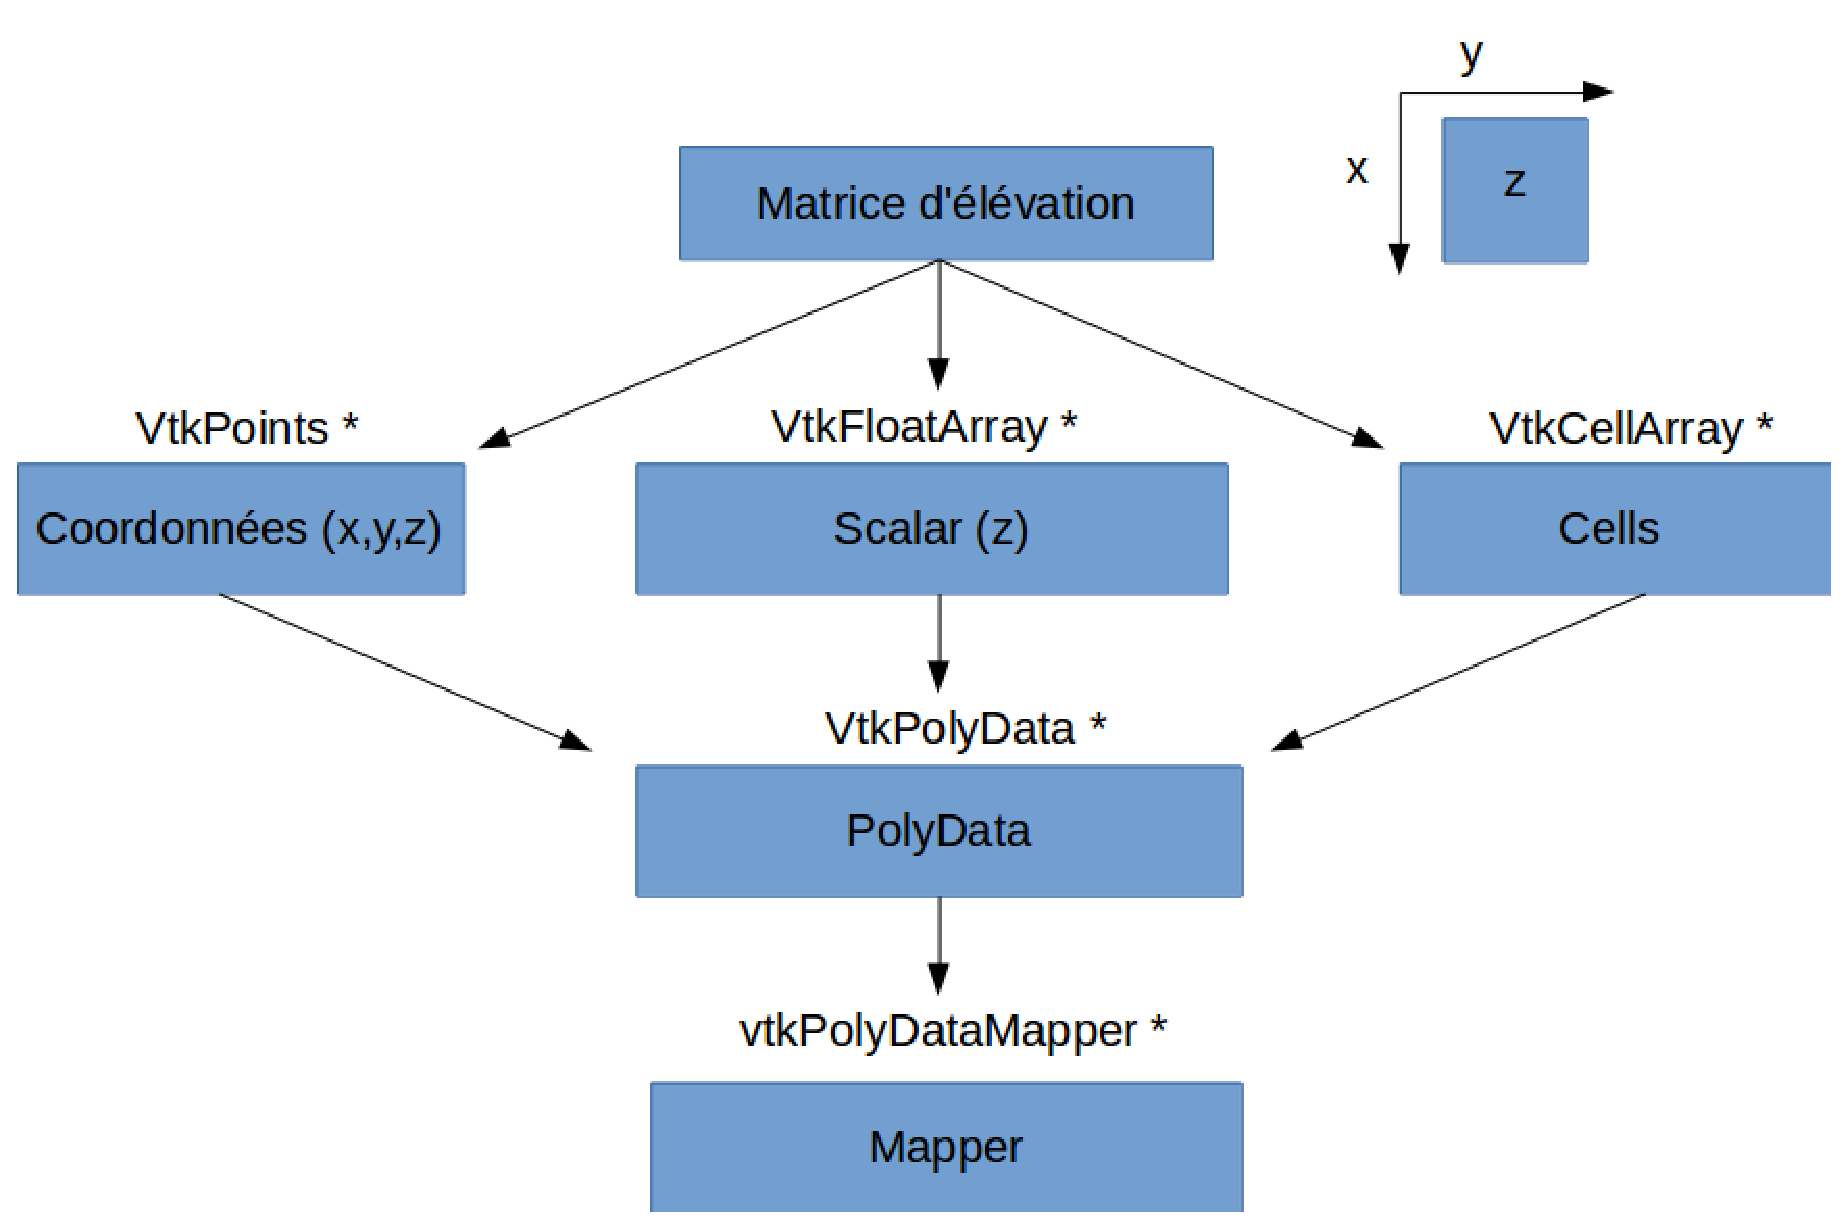
\includegraphics[width=15cm]{VTKMeth.eps}  
	\caption{Construction de l'objet polydataMapper à partir d'une matrice d'élévation. Un schéma de la matrice est représenté en haut à droite de la figure. A partir de cette matrice trois éléments sont extraits : les coordonnées qui sont stockées dans un vtkPoints, les valeurs d'élévations qui sont associées à une couleurs stockée dans un vtkFloatArray et les cellules qui représentent le maillage dans un vtkCellArray. Ces trois éléments sont ensuite associés dans un vtkPolyData qui servira ensuite à construire le mapper.}
	\label{fig:VTKMeth}
\end{figure} 

Pour utiliser VTK, nous pouvons utiliser plusieurs langage tel que le java, le python, le C, le C\# ou encore le C++. Étant donné que les exemples mis à disposition pour android sont codé en C++, j'ai donc utilisé ce langage afin de créer mon propre programme.
	\subsection{Langage de programmation : C++}	
\parindent=1.5em
	Le C++, descendant du C, est un langage de programmation compilé apparu en 1983 et ayant subit plusieurs révisions depuis, dont la dernière était en 2014. Avec lui, nous pouvons programmer sous les paradigmes : 
\begin{itemize}\setlength{\itemsep}{1mm}
	 \item[$\bullet$] procédurale $\rightarrow$ permet de décomposer le code en sous fonctions pouvant être réutilisées plusieurs fois dans le programme voir s'appeler elles-même (récursivité)
	 \item[$\bullet$] orienté objet $\rightarrow$ permet l'utilisation des objets qui sont des ensembles groupé de variables et de méthodes associées à des entités intégrant naturellement ces variables et méthodes.
	 \item[$\bullet$] générique $\rightarrow$ permet la définition d'algorithme identique opérant sur des données de types différents.
\end{itemize}
 
  Pour coder sous ce langage plusieurs choix étaient à ma disposition : un environnement de développement (IDE) ou l'association entre un éditeur de texte et CMAKE (Cross platforme MAKE). 
  
  Dans un premier temps, j'ai utilisé un IDE (code::block) qui est un ensemble d'outils permettant de faciliter le travail du développeur. Il possède donc un éditeur de texte destiné à la programmation, des fonctions permettant de démarrer le compilateur ou l'éditeur de liens par simple pression sur un bouton et un débogueur en ligne. Le débogueur en ligne permet d'exécuter le programme en construction ligne par ligne. 
  
  Dans un deuxième temps, j'ai donc utilisé un éditeur de texte (Sublime text) couplé à CMAKE. Sublime text est un éditeur de texte conçu pour la programmation et CMAKE est un logiciel de compilation multiplateforme. CMAKE va utiliser des fichiers appeler "CMAKELists.txt", communs pour toutes les plateformes, afin de générer des makefiles. Les makefiles sont utilisés par le programme make pour exécuter un ensemble d'actions, comme la compilation d'un projet, l'archivage de document, la mise à jour de site, etc ... Ici on l'utilise pour la compilation du projet en C++.
  
   \vspace{0.25cm}
Comme nous l'avons vu plus haut, le C++ est un langage multiplateforme donc qui permet de construire des applications android.
	\subsection{Programmation mobile}
	Durant mon stage, je me suis concentré sur la partie android des applications mobiles. Pour coder sous android, nous avons besoin d'un environnement de travail adéquat. L'environnement que j'ai utilisé est Android Studio. En effet, 


%%%%%%%%%%%%%%%%%%%%%%%%%%%%%%%%% Résultat %%%%%%%%%%%%%%%%%%%%%%%%%%%%%%%%%%%%%%%%%%%%%%%%%%%%%%%%%%


\newpage
\section{Résultat}
	\subsection{Les classes}
Comme je l'ai dis plus haut, le C++ est un langage de programmation orienté objet. J'ai donc créé plusieurs classes lors de la construction de mon programmes.  

\vspace{0.25cm}
Tout d'abord, nous avons les classes représentant les données de la cornées : DataCornee, ParserTopos et DataPachymetry.
\parindent=0em

\textbf{DataCornee : }
représente les données d'une cornée en leur donnant un nom, comme "Surface anterior", et avec un tableau en deux dimension contenant les données d'élévation de la cornée. 

\textbf{ParserTopos : }
représente les données contenue dans un fichier topos (cf plus haut) grâce à une liste d'objet "DataCornee". Chaque matrice de données peut être appelée séparément avec leur nom, leur numéros ou par des méthodes. Cet objet permet aussi d'afficher les noms des données et contient les rayons des différentes BFS et les coordonnées de leur centres respectifs. Il stocke aussi les coordonnée réelle utilisé en x et en y (de -5 à 5mm par pas de 0.1). 

\textbf{DataPachymetry : } 
reprend les données contenues dans topos afin de reconstruire les données de la pachymétrie. Pour cela, je lui donne soit deux matrices représentant les surfaces antérieures et postérieures de la cornée soit l'objet ParserTopos. Il construit ensuite la matrice de coordonnée qui sera utilisée dans la visualisation de la pachymétrie. Nous verrons cela un peu plus tard.

\vspace{0.25cm}
\parindent=1.5em
Ensuite, nous avons les classes permettant la visualisation de la cornée en utilisant VTK : ColorElevationMap, SurfaceElevationMatrice, SurfaceScalarElevationFromMatrice, PachymetryVisualisation, PachymetryVisualisationFromMatrice, VolumeVisualisation.
\parindent=0em

\textbf{ColorElevationMap : }
permet de stocker les objets VTK utiliser pour la visualisation (vtkPoints, vtkCellArray, vtkFloatArray, vtkPolydata, vtkPolyDataMapper, vtkActor). Elle contient aussi les méthodes nécessaires à la construction des cellules utilisées dans le maillage. Cette classe est la principale, c'est à dire qu'elle sera héritée par les autres classes utilisant VTK.

\textbf{SurfaceElevationMatrice : }
hérite de ColorElevationMap, elle permet la visualisation d'une surface via une matrice d'élévation (surface antérieure ou postérieure de la cornée). Dans cette classe, on ajoute des méthodes permettant d'extraire les coordonnées et les "scalars" à partir d'une matrice car celles-ci ne sont pas présentes dans ColorElevationMap.

\textbf{SurfaceScalarElevationFromMatrice : }
hérite de SurfaceElevationMatrice, elle permet la visualisation d'une surface via 2 !!deux!! matrices. La première est une matrice d'élévation, la deuxième représente les valeurs des différences entre la BFS et sa surface associé. Dans cette classes, j'ai fais en sorte d'adapter une des méthodes de la classe hérité !!heriter ? !!!afin qu'elle prenne en compte les deux matrices au lieu d'une.

\textbf{VolumeVisualisation : }
hérite de ColorElevationMap, elle permet de créer un objet de VTK permettant de donner une impression de volume. Dans cette classe on ajoute toutes les méthodes nécessaires à la construction du volume (cf:plus loin).

\textbf{PachymetryVisualisation : }
hérite de ColorElevationMap, elle permet de visualiser les données de l'objet DataPachymetry.

\textbf{PachymetryVisualisationFromMatrice : }
hérite de ColorElevationMap, permet de visualiser la pachymétrie de la cornée contenue dans un objet ParserTopos.

\vspace{0.25cm}
\parindent=1.5em

 J'ai aussi créé d'autre classes dont certaines représente des notions tel que les points, les triangles ou encore les vecteurs. Les autres classes ne représente pas des objets mais contiennent un ensemble de méthodes utiles dans certain cas. Par exemple, j'ai construit une classe contenant l'ensemble de mes fonctions qui permettent de traiter des variables de type string.
	\subsection{visualisation des faces antérieure et postérieure}
	
	\subsection{Le volume}

	\subsection{La pachymétrie}


\newpage
\section{Discussion}
	\subsection{Organisation de l'application}
	\subsection{Difficulté de la programmation mobile}
	 Séduit par cette application, je l'ai étudié dans l'espoir de pouvoir y baser ma propre application. Malheureusement, cette application n'était plus mise à jours régulièrement. En effet, VTK a décidé d'arrêter son développement afin d'inclure la partie android et ios dans VTK en lui même. Donc une grande partie de mon stage a été de trouver comment porter VTK dans une application android. Peut de documentation peut être trouvé sur ce sujet.!!paragraphe a reformuler!!
	 \subsection{Environnement utilisé pour coder}
J'ai préféré utiliser l'association entre Sublime text et CMAKE. En effet, les exemples de VTK utilisaient déjà CMAKE donc leur "CMAKELists.txt" ont pu me servir de base à la construction de celui de mon projet. De plus, étant débutant en C++ j'ai trouvé que cette manière de faire me permettais de mieux comprendre la construction d'un projet en C++.

\newpage
\section{Conclusion}
	
		
\end{document}
